%% LyX 2.1.3 created this file.  For more info, see http://www.lyx.org/.
%% Do not edit unless you really know what you are doing.
\RequirePackage{fix-cm}
\documentclass[twoside,twocolumn,italian]{article}
\usepackage[T1]{fontenc}
\usepackage[latin9]{inputenc}
\usepackage[landscape]{geometry}
\geometry{verbose,tmargin=1cm,bmargin=1.5cm,lmargin=1cm,rmargin=1cm}
\usepackage{array}
\usepackage{textcomp}
\usepackage{multirow}
\usepackage{amsthm}
\usepackage{amsmath}
\usepackage{amssymb}
\usepackage{fixltx2e}
\usepackage{graphicx}

\makeatletter

%%%%%%%%%%%%%%%%%%%%%%%%%%%%%% LyX specific LaTeX commands.
%% Because html converters don't know tabularnewline
\providecommand{\tabularnewline}{\\}

%%%%%%%%%%%%%%%%%%%%%%%%%%%%%% Textclass specific LaTeX commands.
\numberwithin{equation}{section}
\numberwithin{figure}{section}

%%%%%%%%%%%%%%%%%%%%%%%%%%%%%% User specified LaTeX commands.
\renewcommand{\arraystretch}{2}
\date{Un ringraziamento speciale a Michele Albanese}

\makeatother

\usepackage{babel}
\begin{document}

\title{Formulario Fisica Tecnica - Giulio De Pasquale}

\maketitle
\tableofcontents{}

\newpage{}

\listoftables


\cleardoublepage{}


\section{Termodinamica}


\subsection{Unit� di Misura}
\begin{description}
\item [{Energia~Interna}] $U=[J]$, $\bar{u}=[\frac{J}{Kg}]$;
\item [{Calore}] $Q=[J]$, $\bar{q}=[\frac{J}{Kg}]$;
\item [{Potenza~Termica}] $\dot{Q}=[\frac{J}{s}]=[W]$;
\item [{Lavoro}] $L=[J]$, $\bar{l}=[\frac{J}{Kg}]$;
\item [{Potenza~Meccanica}] $\dot{L}=[\frac{J}{s}]=[W]$;
\item [{Entalpia}] $H=[J]$, $\bar{h}=[\frac{J}{Kg}]$;
\item [{Entropia}] $S=[\frac{J}{\text{\textdegree K}}]$, $\bar{s}=[\frac{J}{Kg\cdot\text{\textdegree K}}]$;
\item [{Temperatura}] $T=[\text{\textdegree}K]$;
\item [{Pressione}] $P=[Pa]$;
\item [{Volume}] $V=[m^{3}]$, $\bar{v}=[\frac{m^{3}}{Kg}]$;
\item [{Massa}] $m=[Kg]$;
\item [{Densit�}] $\rho=[\frac{Kg}{m^{3}}]$;
\item [{Velocit�}] $w=[\frac{m}{s}]$;
\item [{Costante~Universale~dei~Gas}] $R=[\frac{J}{\text{\textdegree K}\cdot kmol}]$,
$R^{*}=\frac{R}{M}=[\frac{J}{Kg\cdot\text{\textdegree K}}]$;
\item [{Calore~Specifico}] $c=[\frac{J}{Kg\cdot\text{\textdegree K}}]$;
\item [{Massa~Molare}] $M=[\frac{Kg}{kmol}]$;
\item [{Portata~Massica}] $\dot{m}=[\frac{Kg}{s}]$;
\item [{Portata~Volumetrica}] $\dot{V}=\dot{m}\bar{v}=[\frac{m^{3}}{s}]$;
\end{description}

\subsection{Conversioni}


\subsubsection{Pressione}
\begin{itemize}
\item $1\,ata=98066,5\,Pa;$
\item $1\,bar=10^{5}\,Pa;$
\item $1\,atm=101325\,Pa;$
\end{itemize}

\subsubsection{Calore}
\begin{itemize}
\item $1\,cal=4,184\,J;$
\end{itemize}

\subsection{Masse Molari}
\begin{itemize}
\item $H=1$;
\item $He=4$;
\item $C=12$;
\item $N=14,\,N_{2}=28$;
\item $O=16,\,O_{2}=32$;
\end{itemize}

\subsection{Generale e Propriet� Gas}

Da tenere sempre presente che
\[
P\bar{v}=R^{*}T
\]
riscrivibile come

\[
PV=nRT
\]


Inoltre, il $I$ principio della termodinamica impone che

\[
\Delta U=\overleftarrow{Q}-\overrightarrow{L}
\]

\begin{itemize}
\item $R=8314,4\frac{J}{\text{\textdegree K}\cdot kmol}$;
\item $n=\frac{m}{M}$ dove $n$ = numero di moli;
\item $c_{p}-c_{v}=R^{*}$, la relazione di Mayer;
\item $\dot{V}=\dot{m}\bar{v}$ con $\dot{V}=$ portata volumetrica;
\end{itemize}

\subsection{Calore, Energia Interna, Entalpia ed Entropia}


\subsubsection{Calore}
\begin{itemize}
\item $Q=mc_{x}\varDelta T$ con $c_{x}=cost$;
\item $Q=mc_{v}\varDelta T$ con $V=cost$;
\item $Q=mc_{p}\varDelta T$ con $P=cost$;
\item $Q=T\Delta S$ con $T=cost$;
\item $\dot{Q}=\dot{m}c_{materiale}\Delta T$;
\end{itemize}

\subsubsection{Energia Interna}
\begin{itemize}
\item $d\bar{u}=c_{v}dT$, se gas perfetto;
\item $d\bar{u}=Tds-Pd\bar{v}$;
\end{itemize}

\subsubsection{Entalpia}
\begin{itemize}
\item $H=U+PV$;
\item $d\bar{h}=c_{p}dT$, se gas perfetto;
\item $d\bar{h}=Tds+\bar{v}dP$;
\item $d\bar{h}=\delta q+\bar{v}dP$;
\end{itemize}

\subsubsection{Entropia}
\begin{itemize}
\item $ds=\frac{\delta q}{T}$, nel caso di un processo reversibile;
\item $\varDelta S=\varDelta S_{\overleftarrow{Q}}+\varDelta S_{irr}$;
\item $ds=c_{v}\frac{dT}{T}+R^{*}\frac{d\bar{v}}{\bar{v}}$$\Rightarrow\Delta S=c_{v}ln(\frac{T_{2}}{T_{1}})+R^{*}ln(\frac{V_{2}}{V_{1}});$ 
\item $ds=c_{p}\frac{dT}{T}-R^{*}\frac{dP}{P}\Rightarrow\Delta S=c_{p}ln(\frac{T_{2}}{T_{1}})-R^{*}ln(\frac{P_{2}}{P_{1}});$
\item $ds=c_{p}\frac{d\bar{v}}{\bar{v}}+c_{v}\frac{dP}{P}\Rightarrow\Delta S=c_{p}ln(\frac{V_{2}}{V_{1}})+c_{v}ln(\frac{P_{2}}{P_{1}});$
\item $\Delta S\geq0$ se il sistema � isolato;
\end{itemize}

\subsubsection{Liquidi}
\begin{itemize}
\item $c_{H_{2}0}=4186\frac{J}{kg\cdot\text{\textdegree K}};$
\item $c=c_{v}=c_{p};$
\item $du=\delta q=cdT\Rightarrow\Delta u=c\Delta T;$
\item $ds=c\frac{dT}{T}\Rightarrow\Delta s=cln(\frac{T_{2}}{T_{1}})$;
\item $v=cost$;
\item $\Delta h=c\Delta T+v\Delta P;$
\end{itemize}

\subsection{Trasformazioni Politropiche}
\begin{itemize}
\item $P\bar{v}^{n}=cost$;
\item $T\bar{v}^{n-1}=cost$;
\item $PT^{\frac{n}{1-n}}=cost$;
\end{itemize}

\subsection{Rendimenti}
\begin{itemize}
\item $\eta_{confronto}=\frac{\eta_{serb-reale}}{\eta_{serb-ideale}};$
\item $\eta_{II_{P}}=\frac{\eta_{reale}}{\eta_{ideale}}=\frac{L_{reale}}{L_{ideale}}$;
\end{itemize}

\subsection{Sistemi Bifase}


\subsubsection{Generale}
\begin{itemize}
\item Le transizioni di fase avvengono con $P=costante$ e $T=costante$;
\item $\begin{cases}
\begin{cases}
x=\ensuremath{\frac{v-v_{l}}{v_{v}-v_{l}};} & con\,x=titolo,\,v=propriet\grave{a}\,estensiva\\
v_{lv}=v_{v}-v_{l}
\end{cases}\\
\mbox{\ensuremath{v=v_{l}+xv_{lv};}}\\
\mbox{\ensuremath{h=h_{l}+xh_{lv};}}\\
\mbox{\ensuremath{s=s_{l}+xs_{lv};}}\\
\mbox{\ensuremath{u=u_{l}+xu_{lv};}}
\end{cases}\mbox{}$
\item $dh=d\overleftarrow{q};$
\end{itemize}

\subsubsection{Liquidi sottoraffreddati}
\begin{itemize}
\item $h\cong h_{l@T}$;
\item $s\cong s_{l@T};$
\end{itemize}

\subsection{Sistemi Aperti}


\subsubsection{Generale}
\begin{itemize}
\item $\dot{m}=\rho w\varOmega$ con $\varOmega=sezione$;
\item $\frac{dE}{dt}=\overleftarrow{\dot{m}}[(\overleftarrow{h}-\overrightarrow{h})+g(\overleftarrow{z}-\overrightarrow{z})+\frac{\overleftarrow{w}^{2}-\overrightarrow{w}^{2}}{2}]+\overleftarrow{\dot{Q}}-\overrightarrow{L}$
con $z=altezza$ e $g=accelerazione\,gravitazionale$;
\item $\frac{dS}{dt}=\overleftarrow{\dot{m}}(\overleftarrow{s}-\overrightarrow{s})+\dot{S_{\overleftarrow{Q}}}+\overrightarrow{\dot{S_{irr}}}$;
\item $\frac{dm}{dt}=\overleftarrow{m}-\overrightarrow{m};$
\end{itemize}

\subsubsection{Macchina Aperta}

Dispositivo adiabatico atto a scambiare lavoro per il quale si ipotizzano
trascurabili le variazioni di energia potenziale e cinetica tra le
sezioni di ingresso e di uscita.
\begin{itemize}
\item $\overleftarrow{\dot{m}}(\overleftarrow{h}-\overrightarrow{h})-\overrightarrow{L}=0$;
\item $\overleftarrow{\dot{m}}(\overleftarrow{s}-\overrightarrow{s})+\dot{S}_{irr}=0$;


\subsubsection{Turbina}
\begin{itemize}
\item $\eta_{isT}=\frac{\overrightarrow{\dot{L}}_{reale}}{\overrightarrow{\dot{L}}_{ideale}}=\frac{(h_{1}-h_{2^{'}})}{(h_{1}-h_{2})}$
con $\eta_{is}=$ rendimento isoentropico;
\end{itemize}

\subsubsection{Compressore / Pompa di Calore}
\begin{itemize}
\item $\eta_{isC}=\frac{\overrightarrow{\dot{L}}_{ideale}}{\overrightarrow{\dot{L}}_{reale}}=\frac{(h_{1}-h_{2})}{(h_{1}-h_{2^{'}})}$;
\end{itemize}
\end{itemize}

\subsubsection{Scambiatore di Calore}

Gli scambiatori sono sistemi aperti stazionari che operano senza scambio
di lavoro per i quali si ipotizzano trascurabili le variazioni di
energia potenziale e cinetica tra le sezioni di ingresso e di uscita.
\begin{itemize}
\item $\overleftarrow{\dot{m}}(\overleftarrow{h}-\overrightarrow{h})+\overleftarrow{\dot{Q}}=0$;
\item $\overleftarrow{\dot{m}}(\overleftarrow{s}-\overrightarrow{s})+\dot{S}_{\overleftarrow{Q}}+\dot{S}_{irr}=0$;
\item $\overleftarrow{\dot{Q}}=\overrightarrow{\dot{Q}}$
\end{itemize}

\subsubsection{Diffusore ($w$ decrescente ) e Ugello ($w$ crescente)}

I diffusori e gli ugelli sono sistemi aperti stazionari che operano
senza scambio di lavoro n� calore per i quali si ipotizzano trascurabili
le variazioni di energia potenziale tra le sezioni di ingresso e di
uscita.
\begin{itemize}
\item $[(\overleftarrow{h}-\overrightarrow{h})+\frac{\overleftarrow{w}^{2}-\overrightarrow{w}^{2}}{2}]=0$;
\item $\overleftarrow{\dot{m}}(\overleftarrow{s}-\overrightarrow{s})+\dot{S}_{irr}=0$;
\end{itemize}

\subsubsection{Valvola di Laminazione}

Le valvole di laminazione sono sistemi aperti stazionari che operano
senza scambio di lavoro n� calore per i quali si ipotizzano trascurabili
le variazioni di energia potenziale e cinetica tra le sezioni di ingresso
e di uscita.
\begin{itemize}
\item $(\overleftarrow{h}-\overrightarrow{h})=0$;
\item $\overleftarrow{\dot{m}}(\overleftarrow{s}-\overrightarrow{s})+\dot{S}_{irr}=0$;
\end{itemize}

\subsection{Macchine Motrici a gas ($\protect\overrightarrow{L}$)}

Converte energia termica in lavoro. 


\subsubsection{Generale}
\begin{itemize}
\item $\eta_{reale}=1-\frac{T_{F}}{T_{C}}-\frac{T_{F}\cdot S_{irr}}{Q_{C}}$
\item $\eta_{rev}=1-\frac{T_{F}}{T_{C}}$;
\item $\Delta S_{irr}=-\frac{\overleftarrow{Q}}{T_{C/F}}+\frac{\overrightarrow{Q}}{T_{C/F}}$
dove $Q$ � riferito alla macchina e $T_{C/F}$ � la temperatura associata
al $Q$ corrispondente;
\end{itemize}

\subsection{Macchine Operatrici a gas ($\protect\overleftarrow{L}$)}

Trasferisce energia termica da uno o pi� serbatoi di calore a temperatura
inferiore a uno o pi� serbatoi di calore a temperatura superiore.

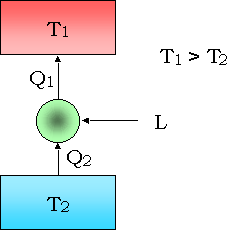
\includegraphics[height=0.25\paperheight]{Formulario/MacchinaOperatrice}
\begin{itemize}
\item $\Delta S_{irr}=-\frac{\overleftarrow{Q}}{T_{C/F}}+\frac{\overrightarrow{Q}}{T_{C/F}}$
dove $Q$ � riferito alla macchina e $T_{C/F}$ � la temperatura associata
al $Q$ corrispondente;
\end{itemize}

\subsubsection{Macchine frigorifere}
\begin{itemize}
\item $L_{rev}=Q_{F}(\frac{T_{C}}{T_{F}}-1)=\frac{Q_{F}}{\varepsilon}$;
\item $L_{reale}=L_{rev}+T_{C}S_{irr}$;
\item $\varepsilon_{f}=\frac{Q_{F}}{L}=\frac{T_{F}}{T_{C}-T_{F}+\frac{T_{C}T_{F}S_{irr}}{\overleftarrow{Q}}}$
;
\item $\varepsilon_{f_{rev}}=\frac{T_{F}}{T_{C}-T_{F}}$;
\end{itemize}

\subsubsection{Macchine calorifere (pompe di calore)}
\begin{itemize}
\item $L_{rev}=Q_{C}(1-\frac{T_{F}}{T_{C}})=\frac{Q_{C}}{\varepsilon}$;
\item $L_{reale}=L_{rev}+T_{F}S_{irr}$;
\item $\varepsilon_{pdc}=\frac{Q_{C}}{L}=\frac{\overrightarrow{Q}+L}{L}=\varepsilon_{f}+1=\frac{T_{C}}{T_{C}-T_{F}+\frac{T_{C}T_{F}S_{irr}}{\overleftarrow{Q}}}$;
\item $\varepsilon_{pdc_{rev}}=\frac{T_{C}}{T_{C}-T_{F}}$;
\end{itemize}

\section{Cicli}


\subsubsection{Generale}
\begin{itemize}
\item $\eta=\frac{L_{netto}}{\overleftarrow{Q}};$
\item $n=\frac{c_{p}}{c_{v}};$
\end{itemize}

\subsection{Cicli simmetrici}

Per i cicli simmetrici valgono le seguenti propriet�:

\[
\bar{v}_{1}\bar{v}_{3}=\bar{v}_{2}\bar{v}_{4}
\]


\[
P_{1}P_{3}=P_{2}P_{4}
\]


\[
T_{1}T_{3}=T_{2}T_{4}
\]



\subsection{Cicli a Gas}


\subsubsection{Sistemi chiusi}
\begin{itemize}
\item $\Delta u=\overleftarrow{q}-\overrightarrow{l};$
\end{itemize}

\paragraph{Carnot a Gas}

Il ciclo di Carnot � costituito da due isoentropiche e due isoterme.

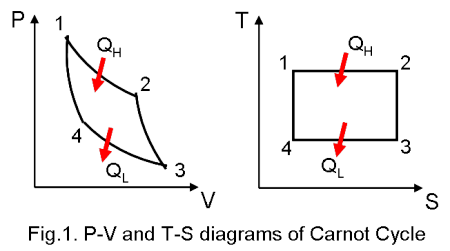
\includegraphics[height=0.25\paperheight]{Formulario/CarnotPVTS}
\begin{itemize}
\item $S_{irr}=-\frac{\overleftarrow{Q}}{T_{C}}+\frac{\overrightarrow{Q}}{T_{F}}$;
\item $\varDelta S=\frac{\overleftarrow{Q}}{T_{2}}=\frac{\overrightarrow{Q}}{T_{1}}$;
\item $\eta_{rev}=1-\frac{T_{1}}{T_{3}}$;
\end{itemize}

\paragraph{Diesel}

Il ciclo Diesel � costituito da due isoentropiche, una isocora ed
una isobara.

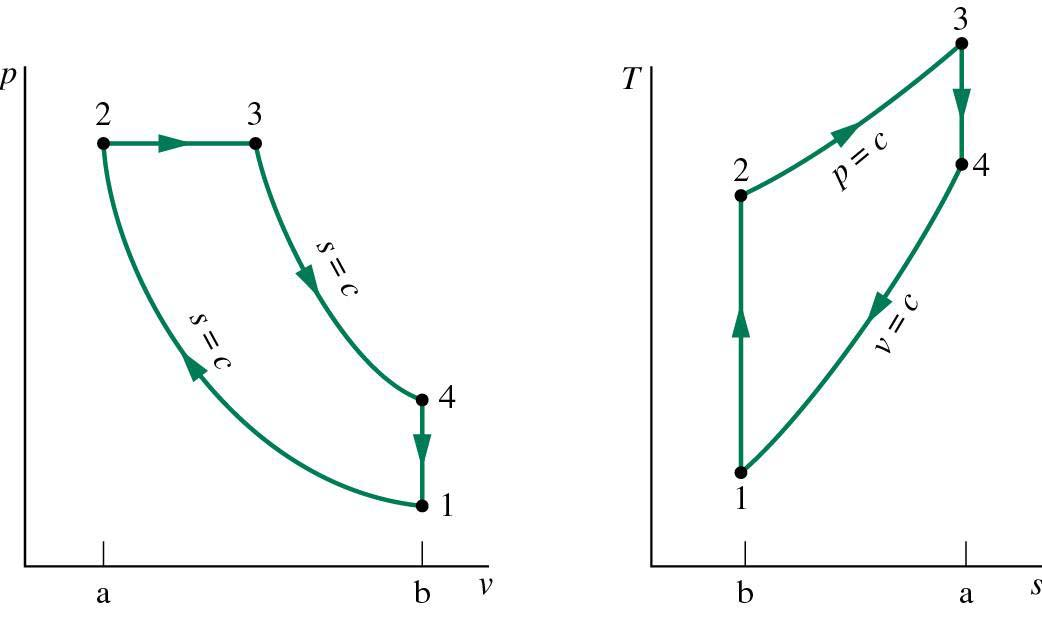
\includegraphics[width=0.5\linewidth,height=0.25\paperheight,keepaspectratio]{Formulario/Diesel}
\begin{itemize}
\item $\eta_{D}=1-\frac{c_{v}T_{1}(\frac{T_{4}}{T_{1}}-1)}{c_{p}T_{2}(\frac{T_{3}}{T_{2}}-1)}$;
\item $\eta=1-\frac{T_{4}-T_{1}}{n(T_{3}-T_{2})}$;
\item $\eta=1-\frac{1}{r^{n-1}}\cdot[\frac{z^{n}-1}{n(z-1)}]$;
\item $r=\frac{V_{1}}{V_{2}}$, rapporto di compressione volumetrico;
\item $z=\frac{V_{3}}{V_{2}}$, rapporto di combustione;
\end{itemize}

\paragraph{Otto}

Ciclo simmetrico costituito da due isoentropiche e due isocore.

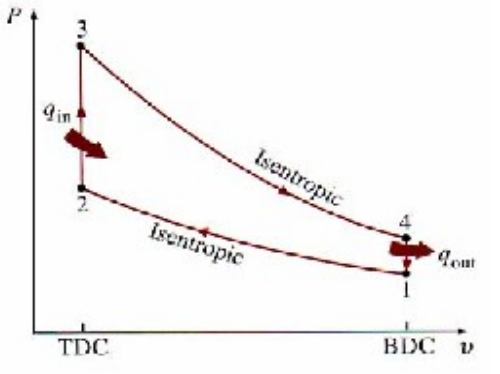
\includegraphics[width=0.5\linewidth,height=0.25\paperheight,keepaspectratio]{Formulario/OttoPV.PNG}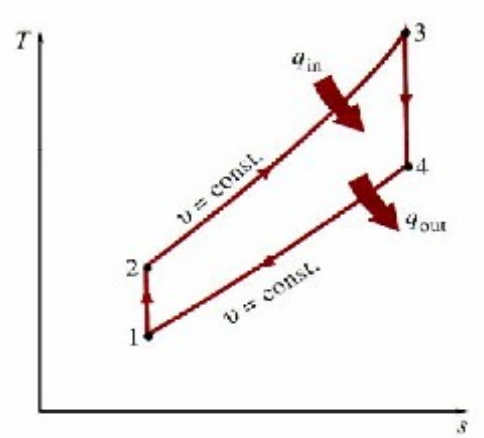
\includegraphics[width=0.5\linewidth,height=0.25\paperheight,keepaspectratio]{Formulario/OttoTS.PNG}
\begin{itemize}
\item $\overleftarrow{Q}=u_{3}-u_{2}=c_{v}(T_{3}-T_{2})$;
\item $\overrightarrow{Q}=u_{4}-u_{1}=c_{v}(T_{4}-T_{1})$;
\item $l=c_{v}(T_{3}-T_{4})-c_{v}(T_{2}-T_{1})=c_{v}T_{3}(1-\frac{1}{r_{vol}^{n-1}})-c_{v}T_{1}(r_{vol}^{n-1}-1)=c_{v}T_{3}(1-\frac{T_{4}}{T_{3}})-c_{v}T_{1}(\frac{T_{2}}{T_{1}}-1)$;
\item $\eta=1-\frac{T_{1}}{T_{2}}=1-r_{vol}^{1-n};$
\item $r_{vol}=\frac{V_{1}}{V_{2}}$;
\end{itemize}

\subsubsection{Sistemi aperti}
\begin{itemize}
\item $\Delta h=\overleftarrow{q}-\overrightarrow{l};$
\end{itemize}

\paragraph{Joule-Brayton}

Il ciclo Joule-Brayton � un ciclo simmetrico ed un sistema aperto
costituito da due isoentropiche e due isobare.

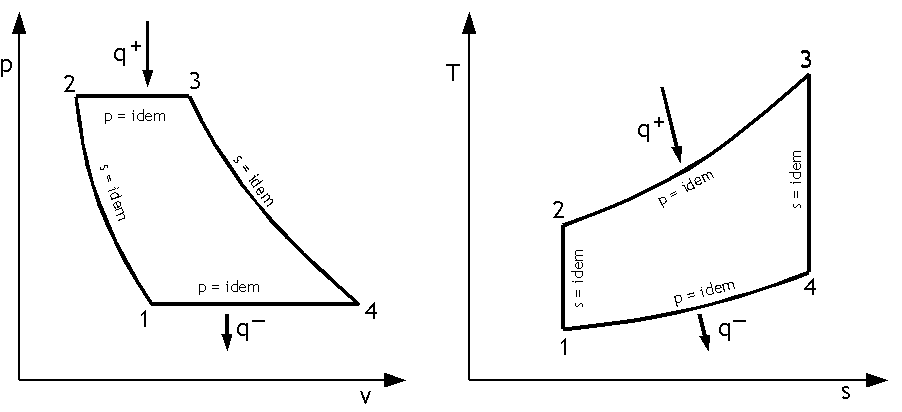
\includegraphics[width=0.5\linewidth,height=0.25\paperheight,keepaspectratio]{Formulario/Brayton_pvTs}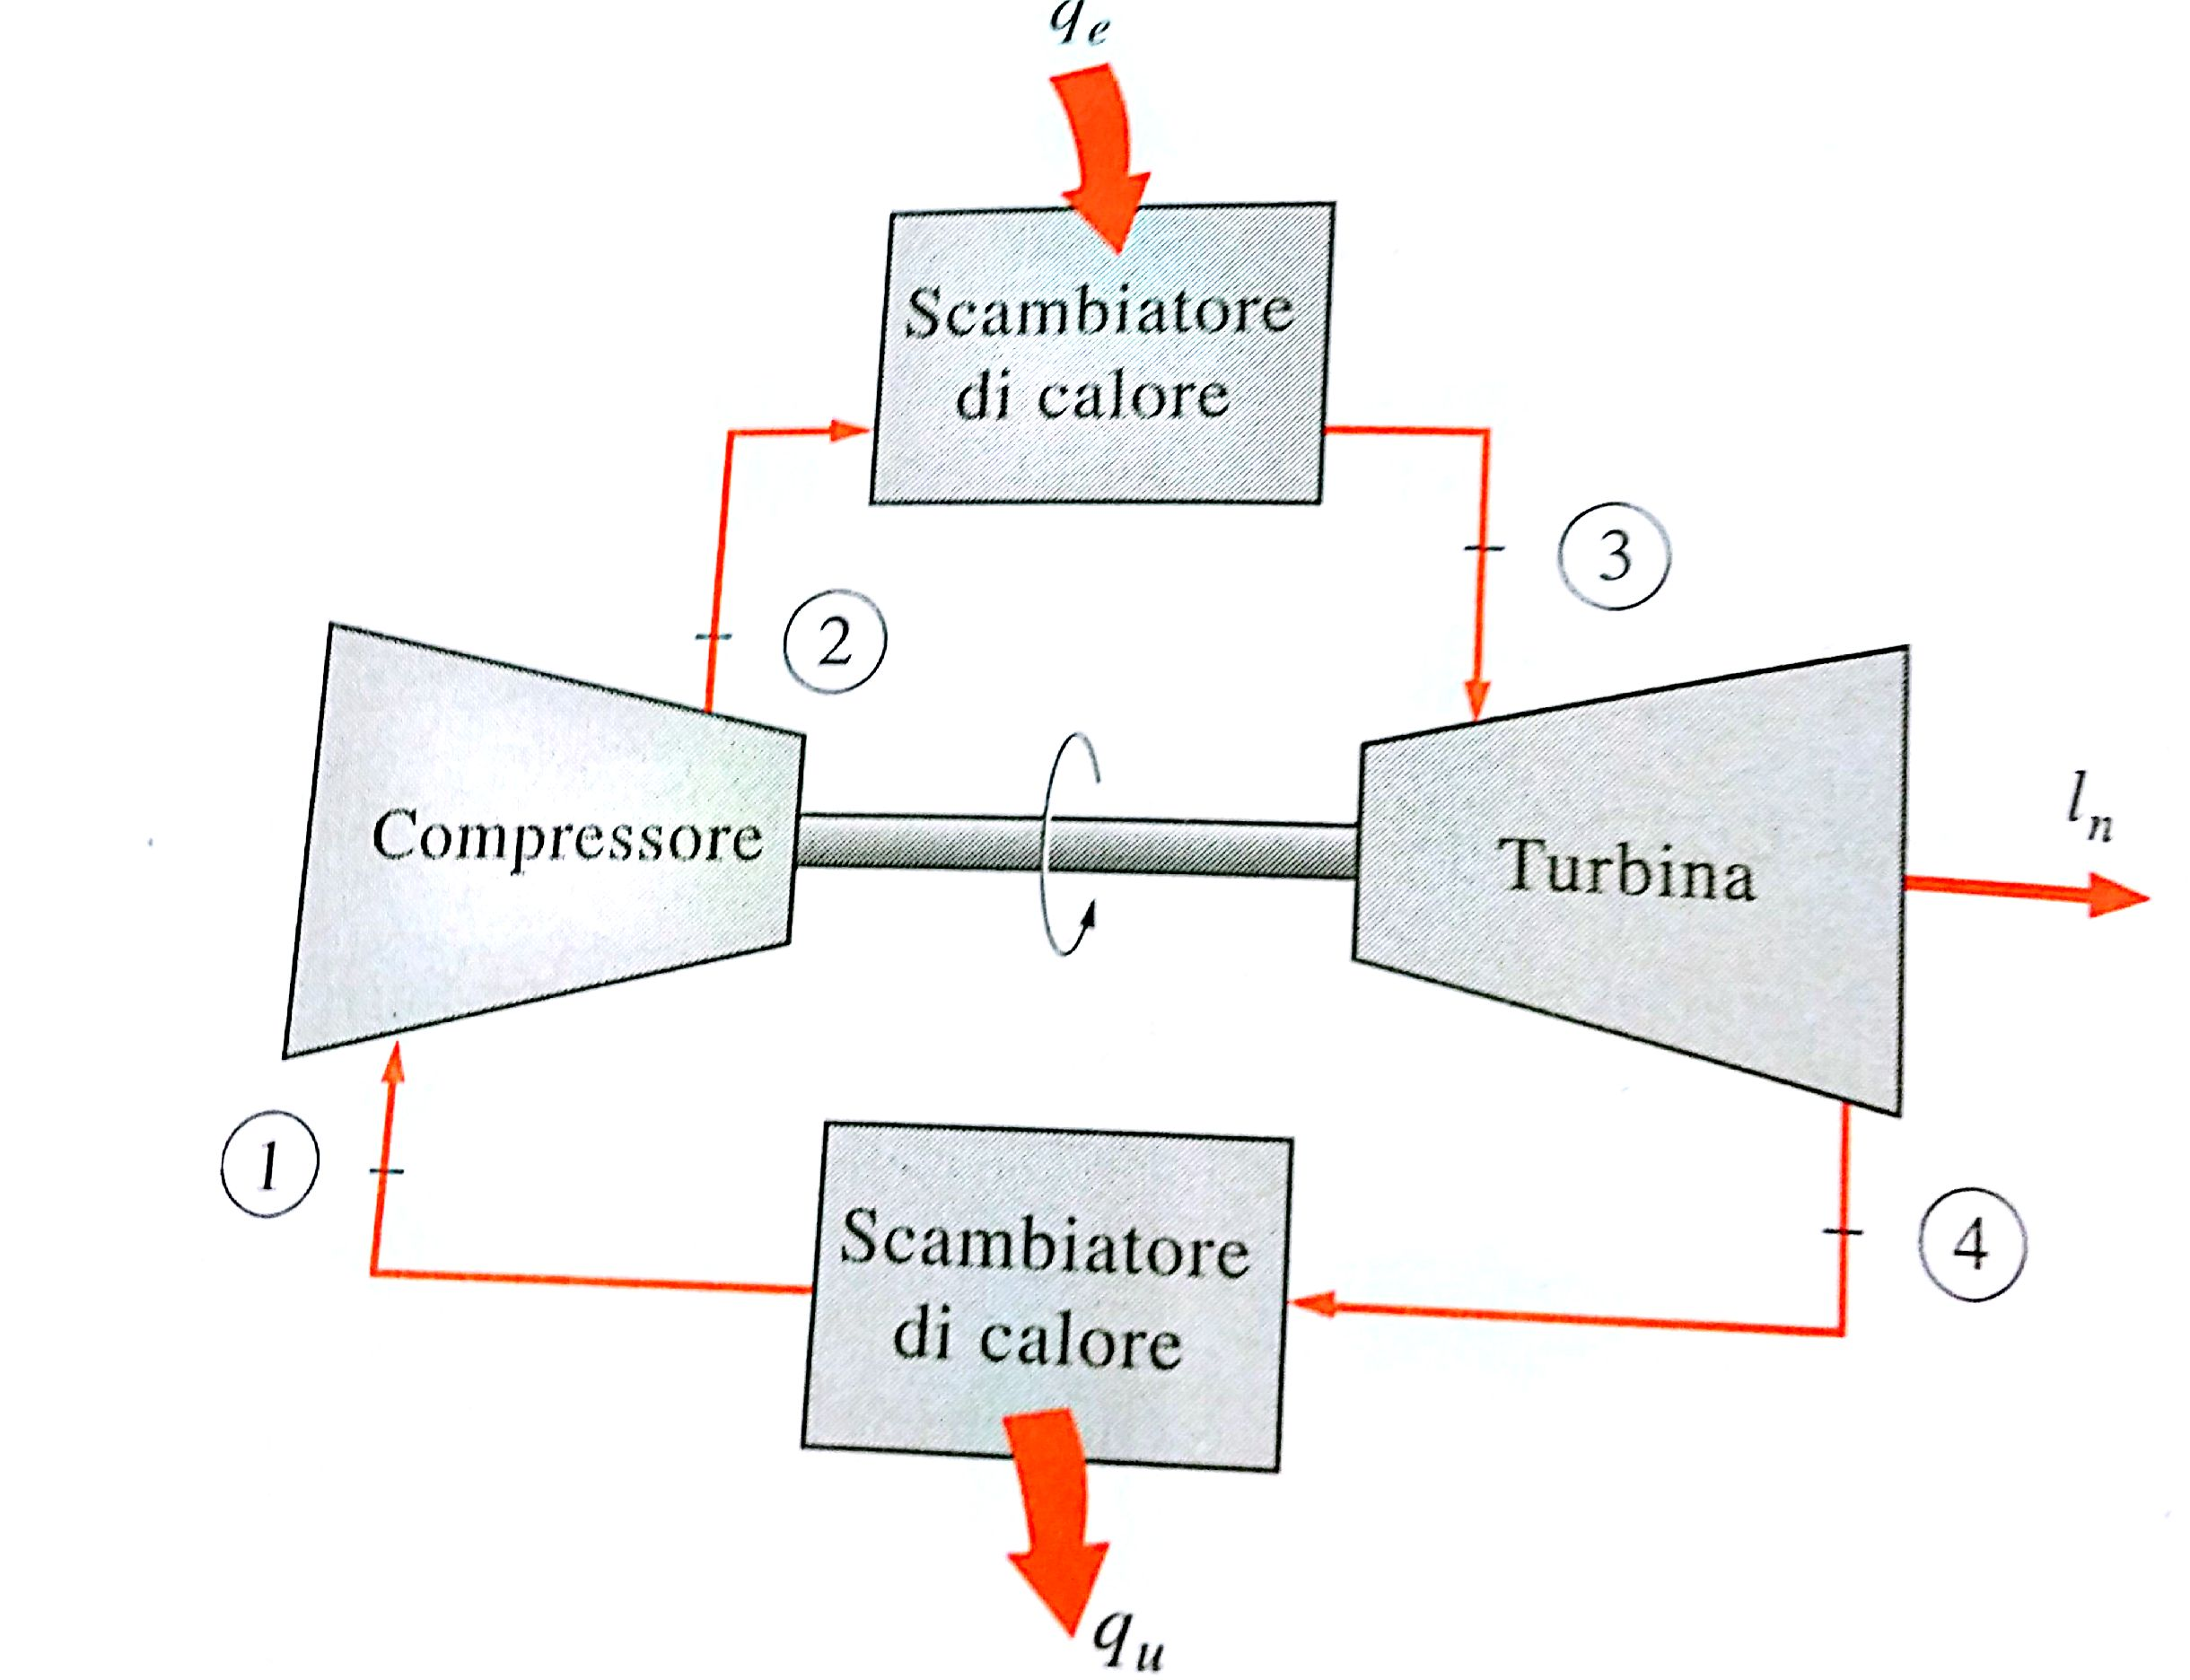
\includegraphics[width=0.5\linewidth,height=0.25\paperheight]{Formulario/JBComp}
\begin{itemize}
\item $\overleftarrow{Q}=\dot{m}(h_{3}-h_{2})=\dot{m}c_{p}(T_{3}-T_{2})$;
\item $\overrightarrow{Q}=\dot{m}(h_{4}-h_{1})=\dot{m}c_{p}(T_{4}-T_{1})$;
\item $l=c_{p}(T_{3}-T_{4})-c_{p}(T_{2}-T_{1})=c_{p}T_{3}(1-\frac{T_{4}}{T_{3}})-c_{p}T_{1}(\frac{T_{2}}{T_{1}}-1)$;
\item $\eta_{JB}=1-\frac{T_{1}}{T_{2}}=1-\frac{1}{r^{\frac{n-1}{n}}}$;
\item $r=\frac{P_{2}}{P_{1}}$ con $r=$ rapporto di compressione;
\item $r_{pmin}=1$;
\item $r_{pmax}=(\frac{T_{3}}{T_{1}})^{\frac{n}{n-1}}$;
\end{itemize}
Affinch� si possa operare una rigenerazione bisogna che la temperatura
di fine espansione sia maggiore della temperatura di fine compressione.


\subsection{Cicli a Vapore}


\subsubsection{Generale}
\begin{itemize}
\item $\Delta h=\overleftarrow{q}-\overrightarrow{l};$
\end{itemize}

\subsubsection{Cicli diretti}


\paragraph{Carnot\protect \\
}

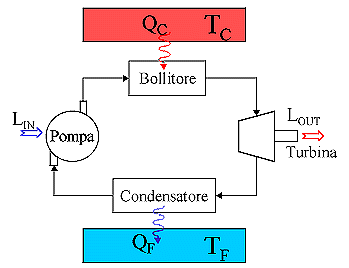
\includegraphics[width=0.33\linewidth,height=0.25\paperheight,keepaspectratio]{Formulario/CarnotVapore}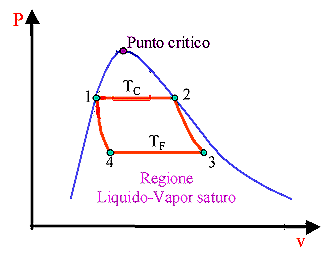
\includegraphics[width=0.33\linewidth,height=0.25\paperheight,keepaspectratio]{Formulario/CarnotVaporePV}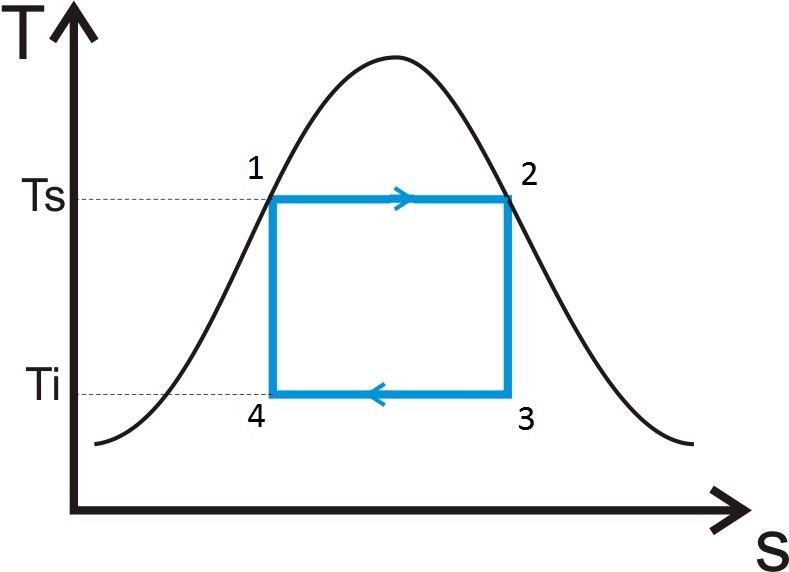
\includegraphics[width=0.33\linewidth,height=0.25\paperheight,keepaspectratio]{Formulario/CarnotVaporeTS}


\paragraph{Rankine Semplice}

L'acqua entra nella pompa $(1)$ come liquido saturo. Entra in caldaia,
a $P=cost$, $(2)$ come liquido sottoraffreddato ed esce come vapore
surriscaldato in $(3)$. Il vapore surriscaldato entra in turbina
$(3)$ e si espande isoentropicamente; la pressione e la temperatura
scendono sino ad arrivare in $(4)$ dove si trova una miscela satura
di liquido e vapore ad elevato titolo. Il vapore entra nel condensatore
$(4)$ e viene condensato a $P=cost$ uscendo come liquido saturo.
\begin{itemize}
\item $(1)\rightarrow(2)\,\,\,\Delta S=0$;
\item $(2)\rightarrow(3)\,\,\,P=cost$;
\item $(3)\rightarrow(4)\,\,\,\Delta S=0$;
\item $(4)\rightarrow(1)\,\,\,P=cost,\,T=cost$;
\end{itemize}
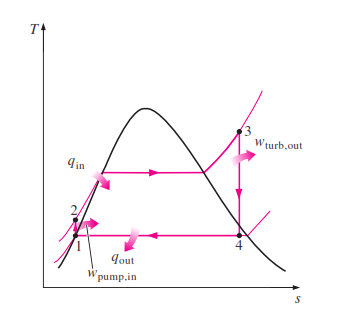
\includegraphics[width=0.5\linewidth,height=0.25\paperheight,keepaspectratio]{Formulario/6894054_orig}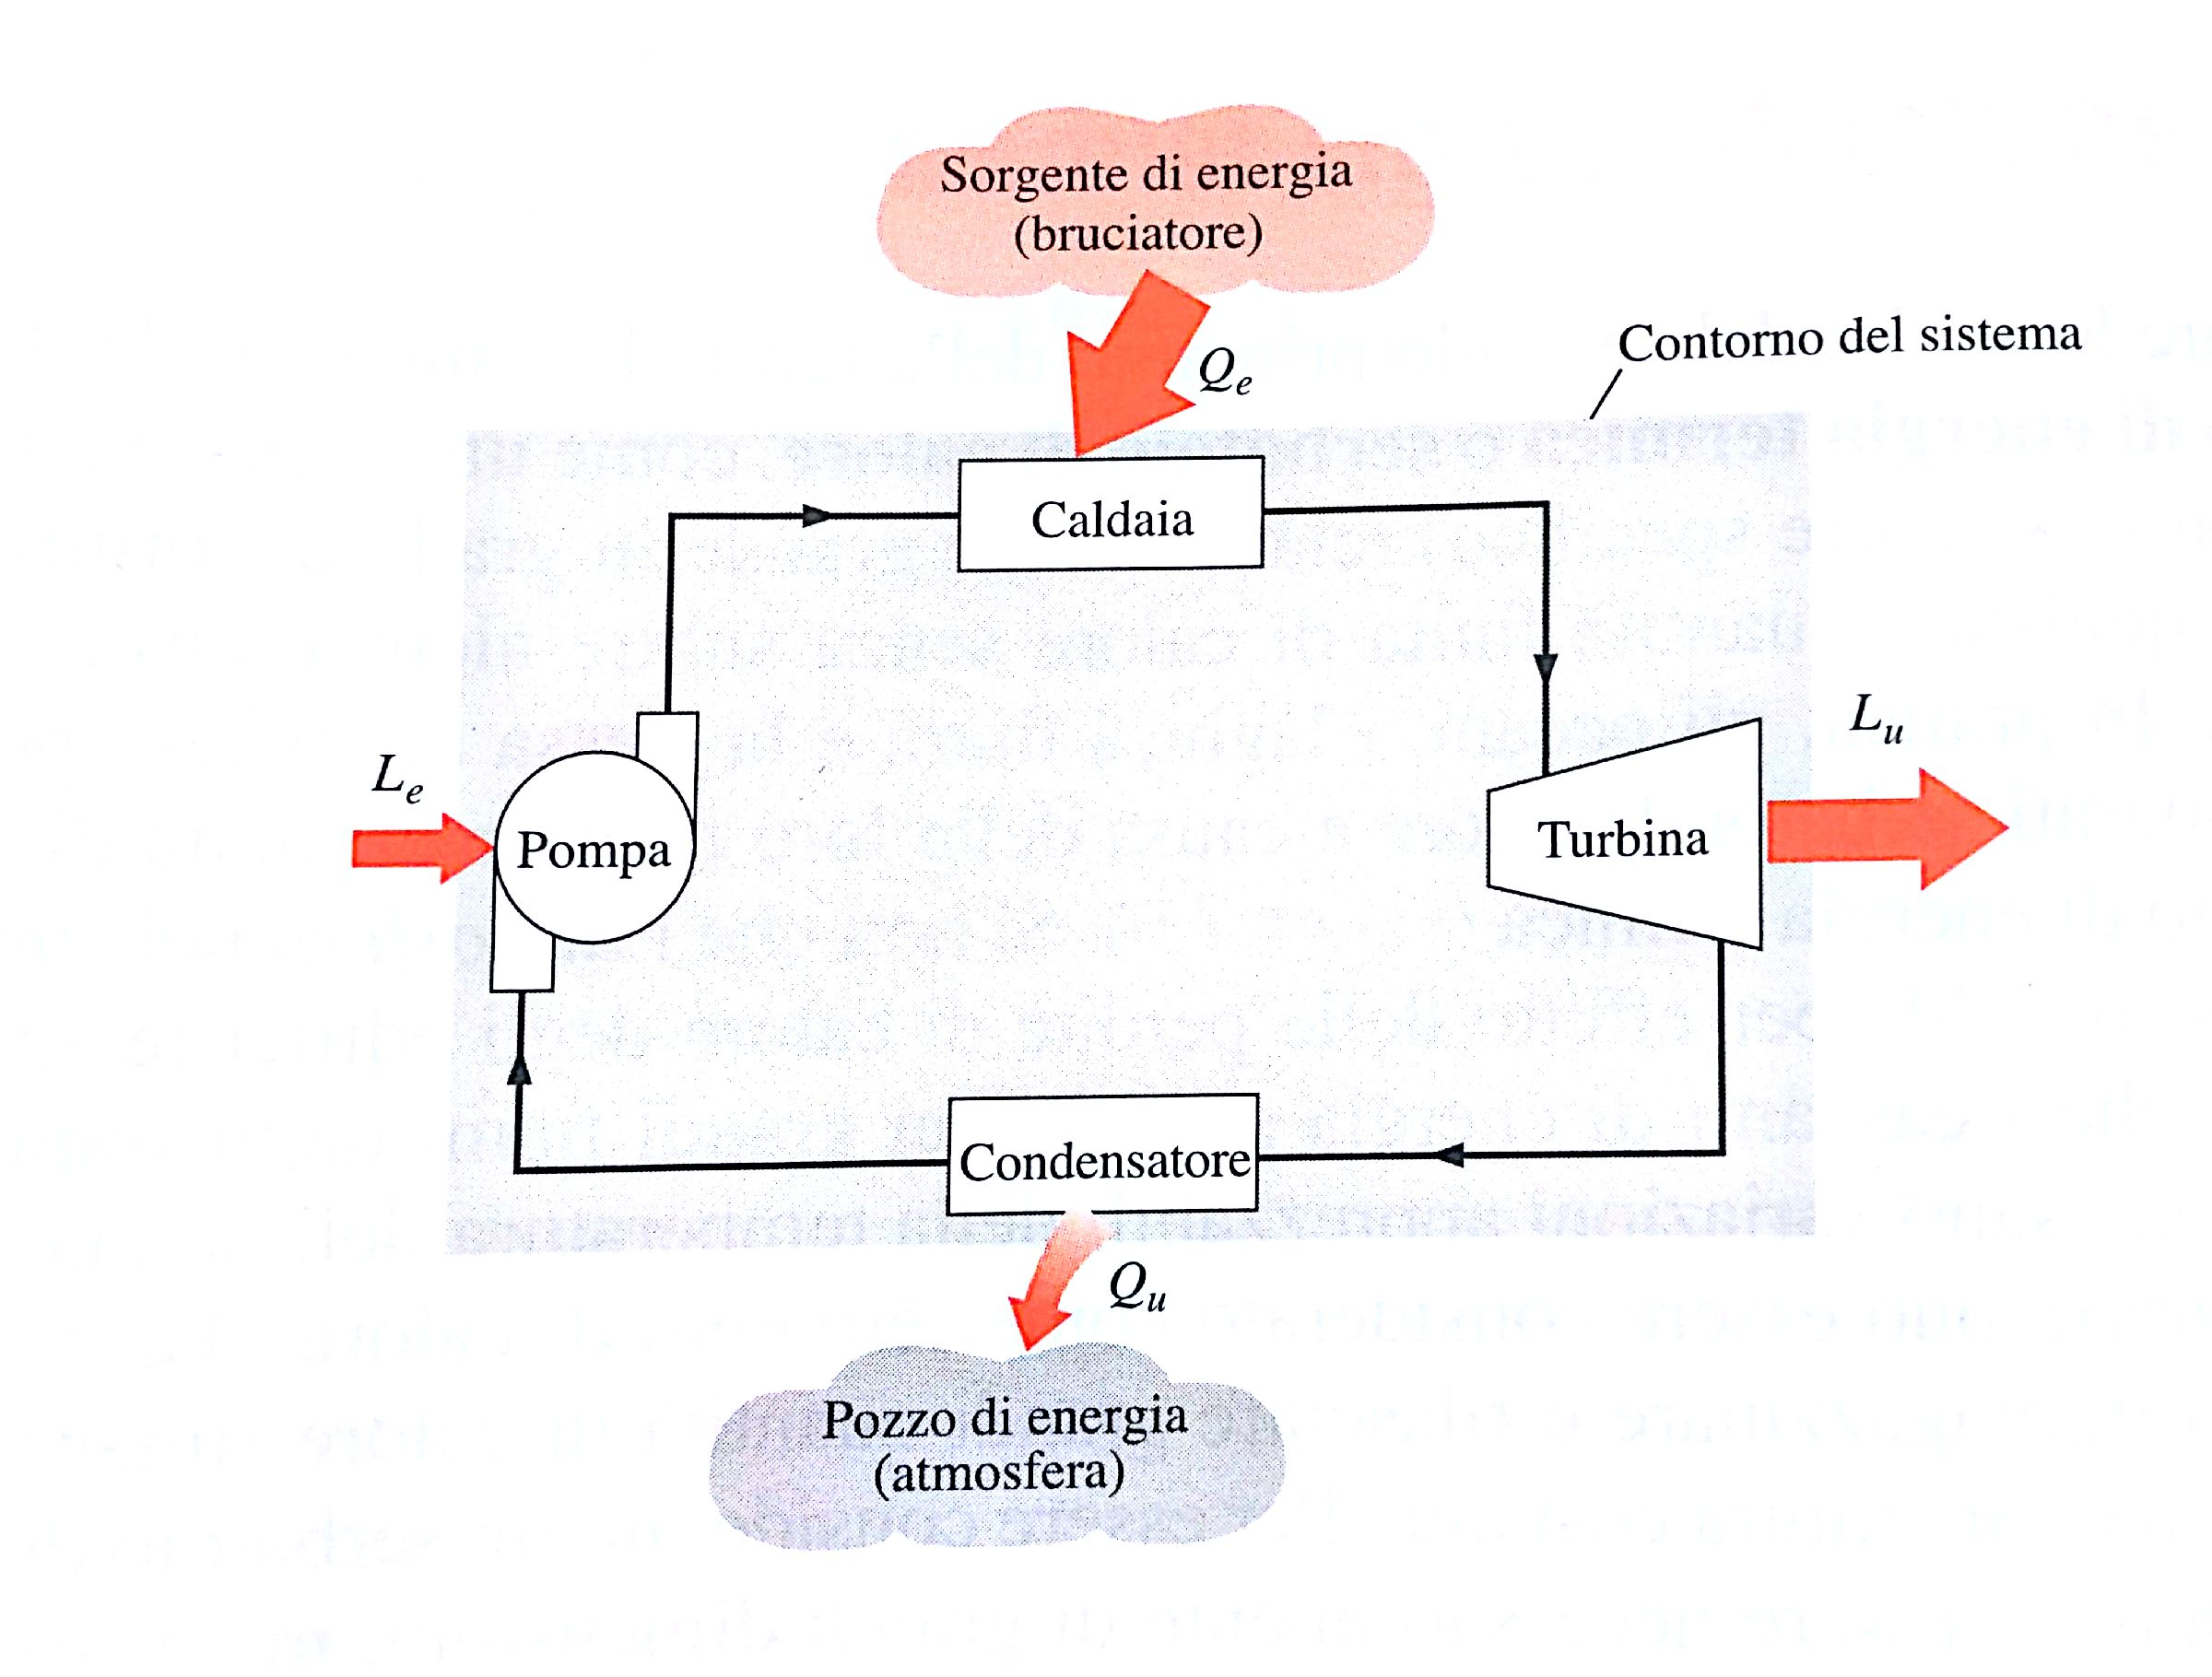
\includegraphics[width=0.5\linewidth,height=0.25\paperheight,keepaspectratio]{Formulario/RankineComp}


\paragraph{Rankine con surriscaldamento}

In aggiunta alle fasi di un ciclo Rankine semplice si ha un'espansione
isoentropica in una turbina ad alta pressione $(3\rightarrow4)$,
un surriscaldamento $(4\rightarrow5)$ ed un'espansione isoentropica
in una turbina a bassa pressione $(5\rightarrow6)$:
\begin{itemize}
\item $(1)\rightarrow(2)\,\,\,\Delta S=0$;
\item $(2)\rightarrow(3)\,\,\,P=cost$;
\item $(3)\rightarrow(4)\,\,\,\Delta S=0$;
\item $(4)\rightarrow(5)\,\,\,P=cost$;
\item $(5)\rightarrow(6)\,\,\,\Delta S=0$;
\item $(6)\rightarrow(1)\,\,\,P=cost,\,T=cost$;
\end{itemize}
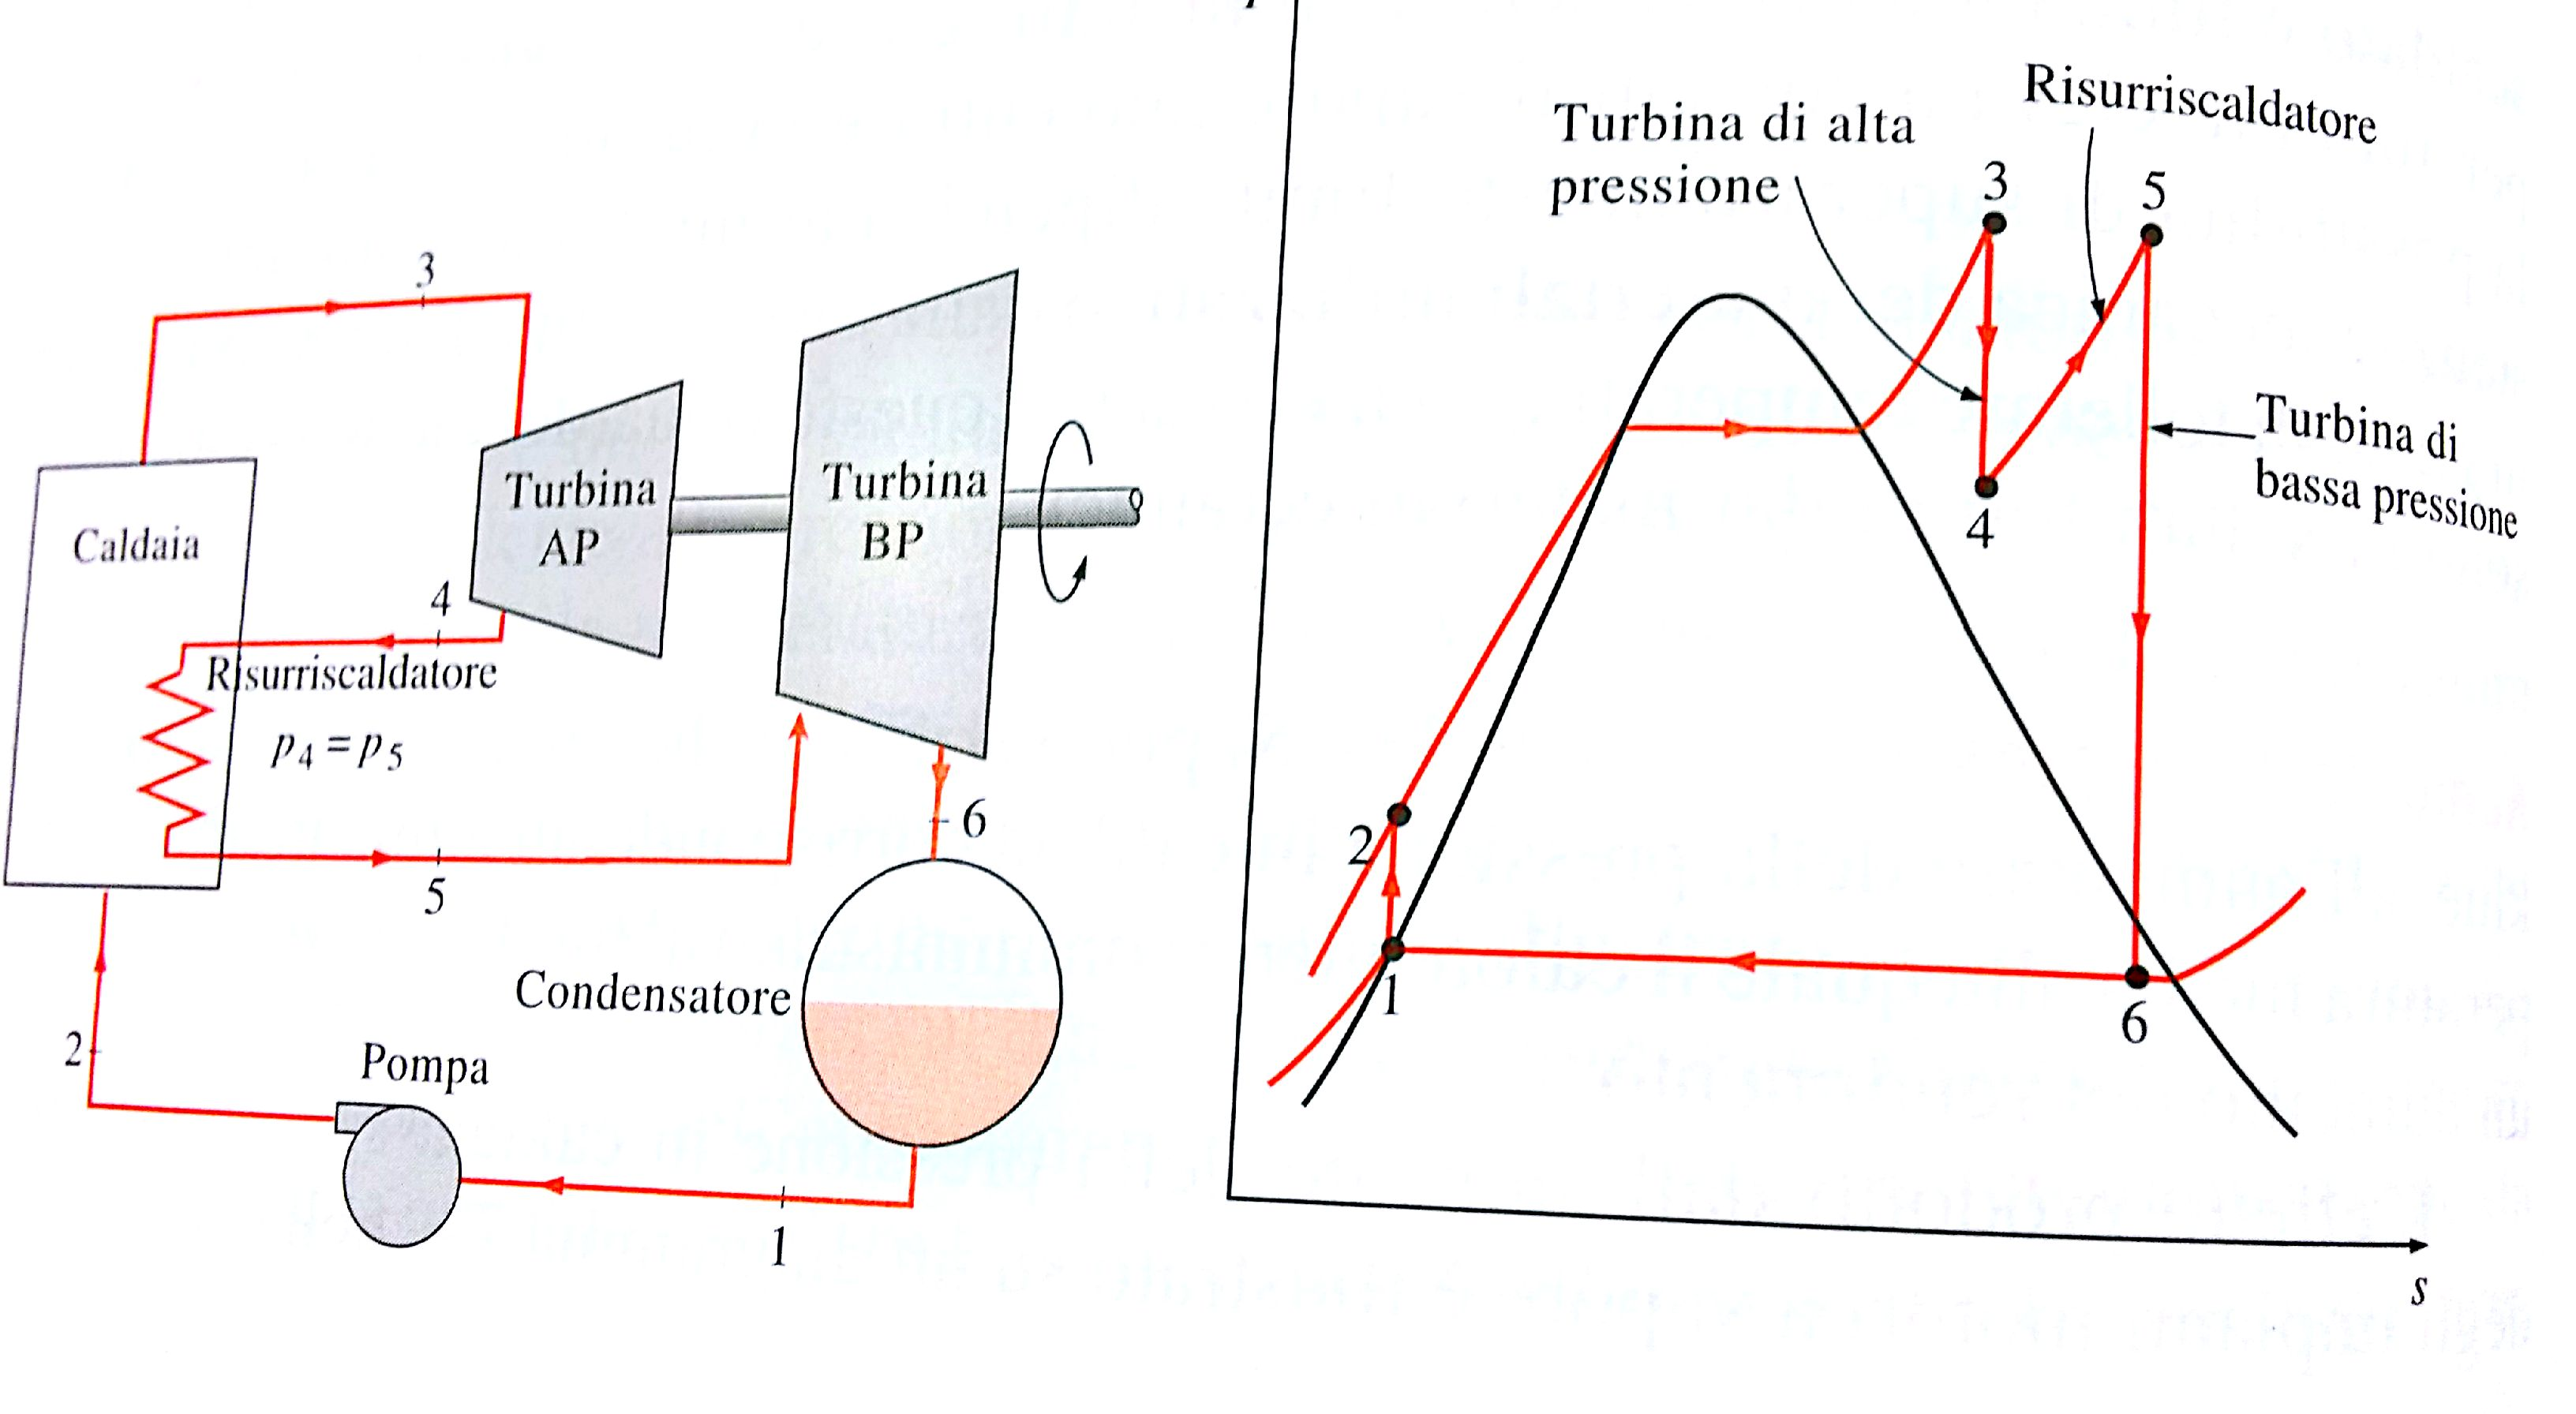
\includegraphics[width=0.5\linewidth,height=0.25\paperheight,keepaspectratio]{Formulario/RankineSurriscaldamento}


\subsubsection{Cicli indiretti}


\paragraph{Carnot inverso\protect \\
}

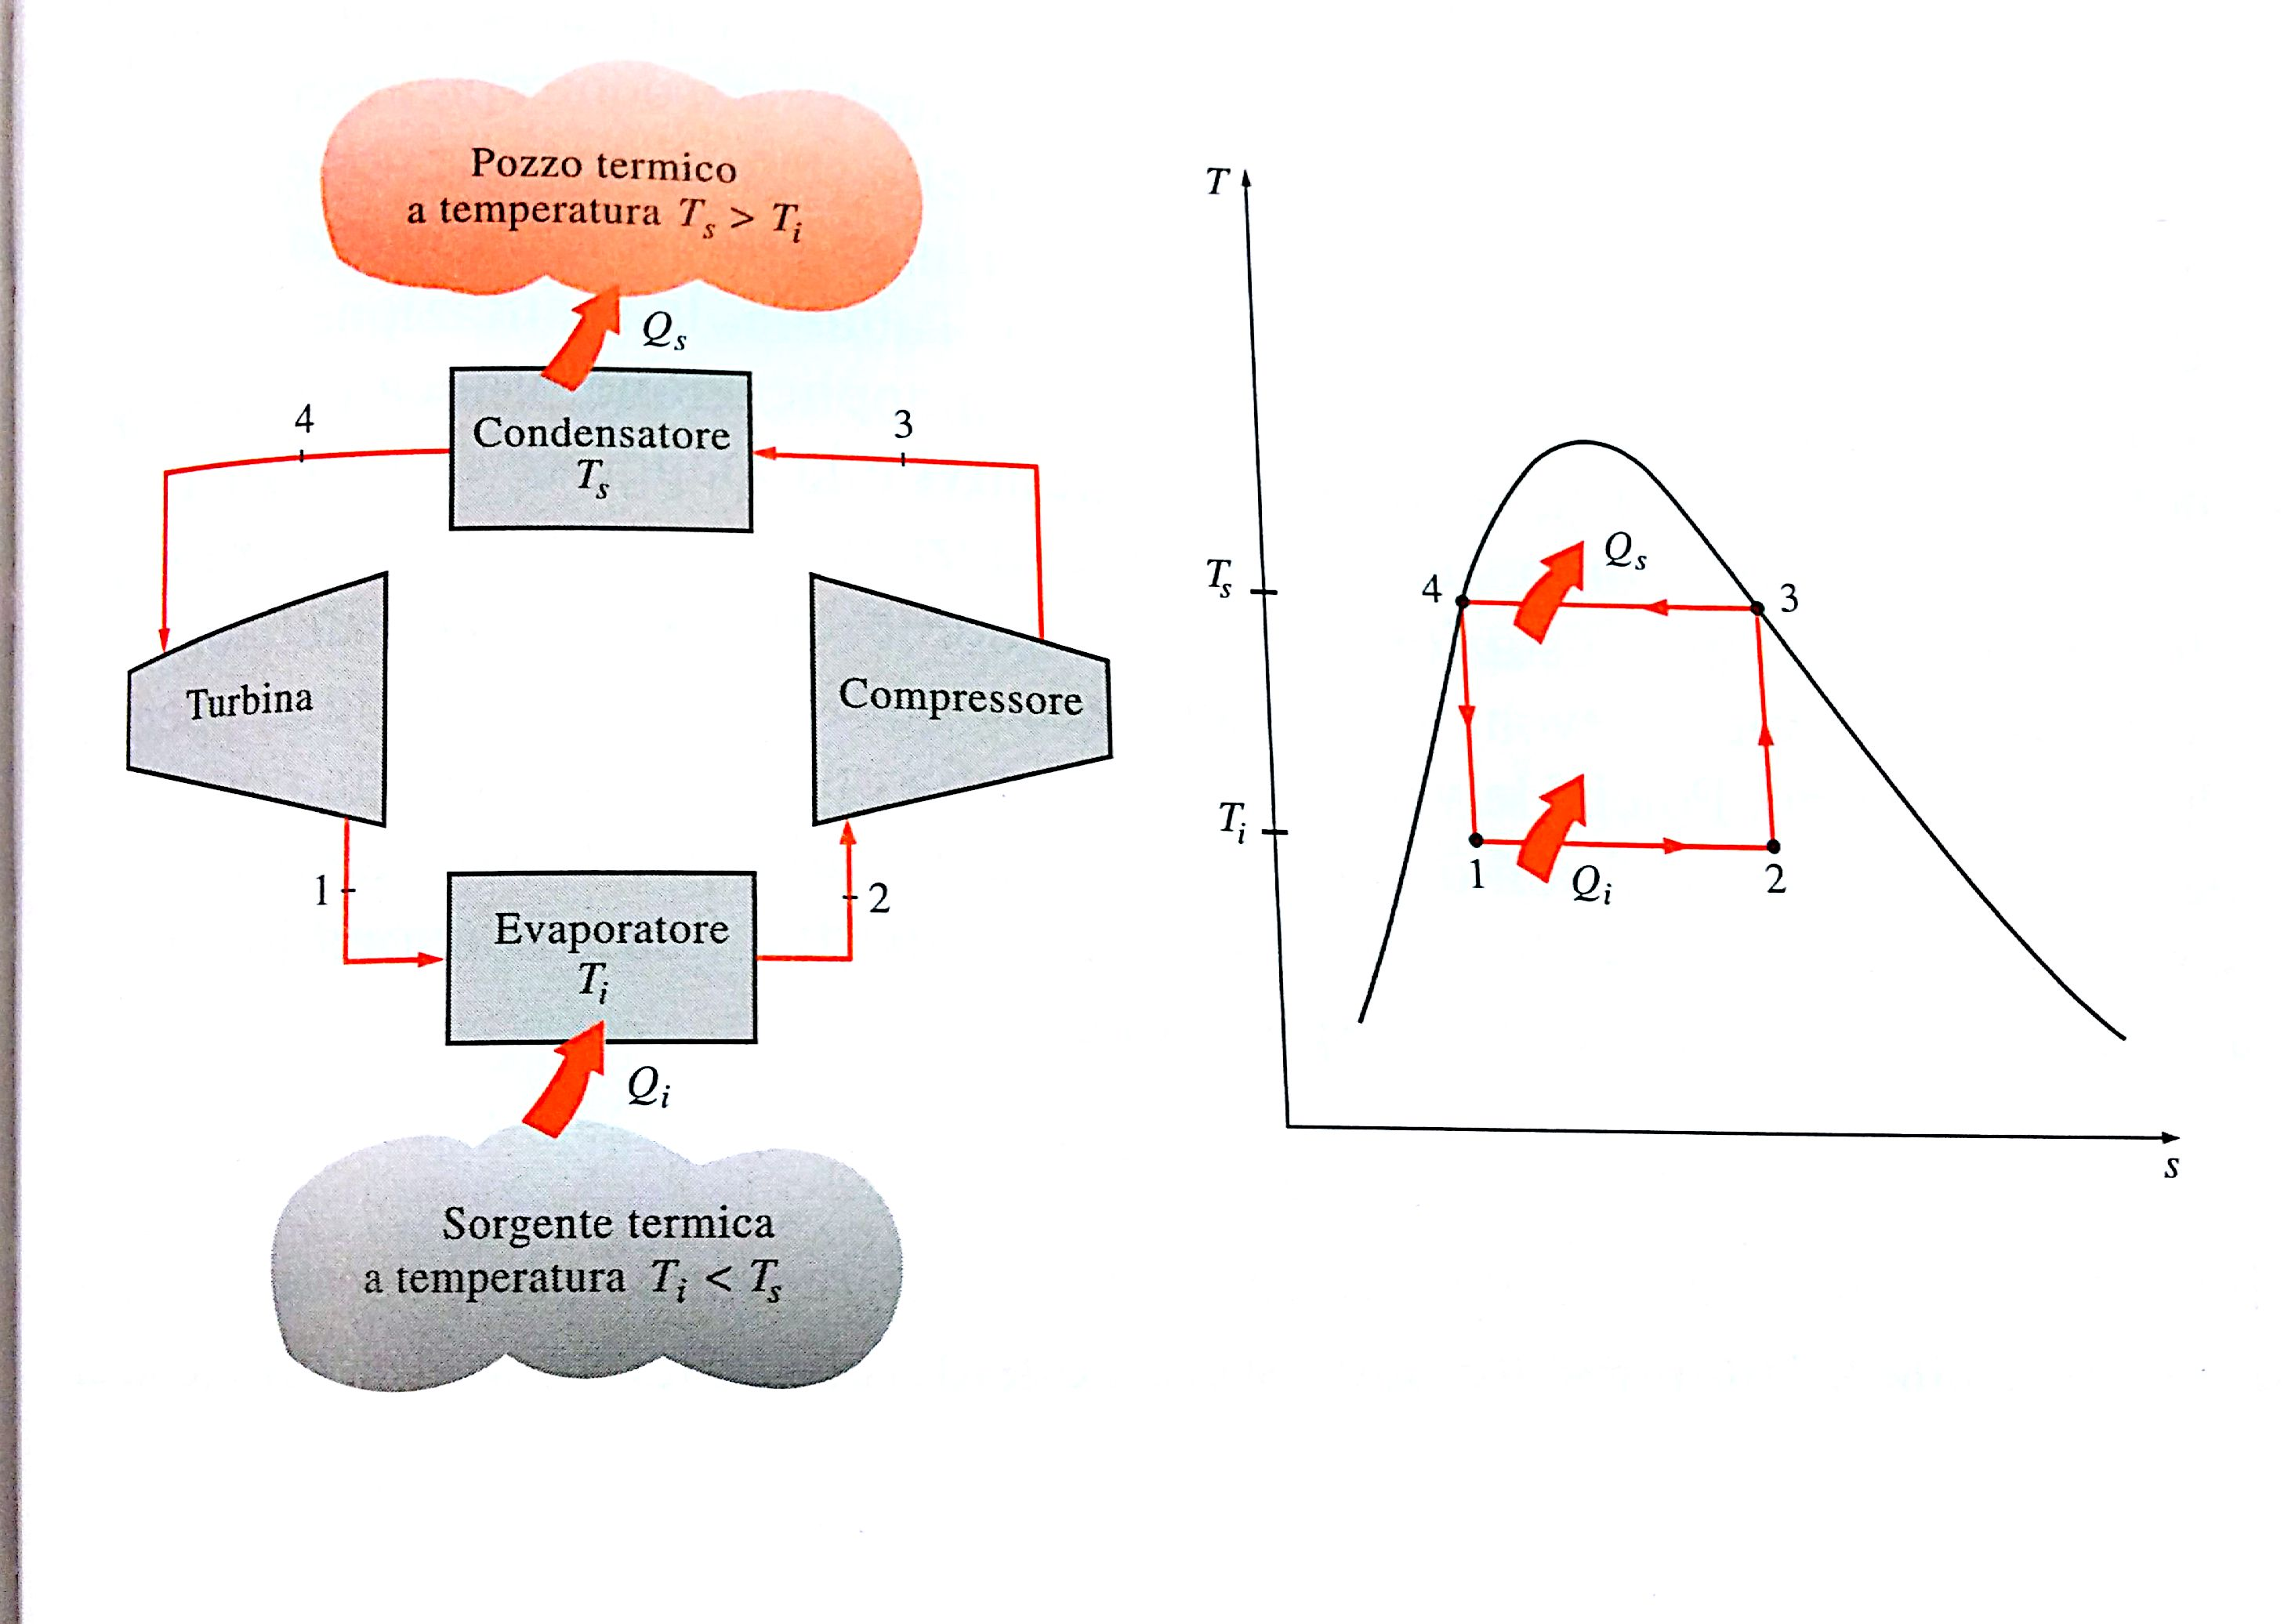
\includegraphics[width=0.5\linewidth,height=0.25\paperheight,keepaspectratio]{Formulario/CarnotVaporeInverso}


\paragraph{Ciclo inverso a compressione di vapore ideale\protect \\
}

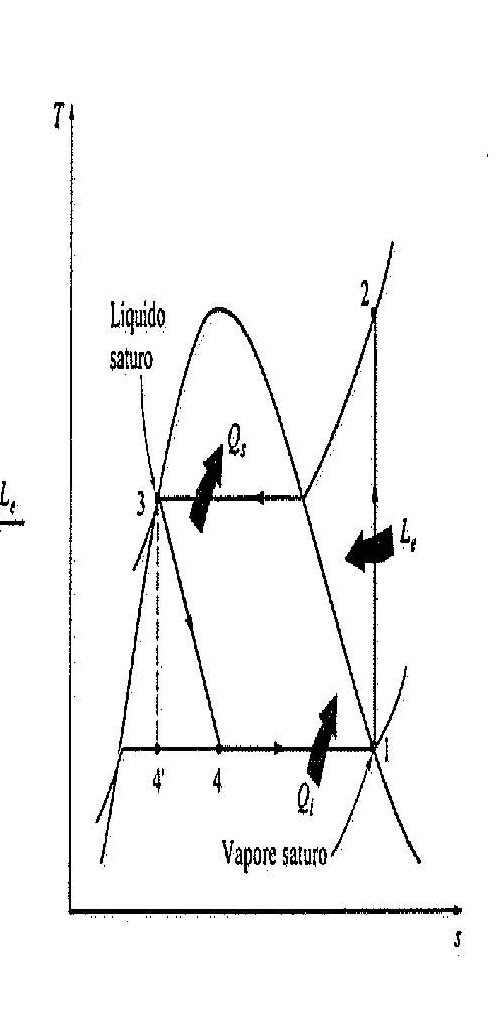
\includegraphics[width=0.5\linewidth,height=0.35\paperheight,keepaspectratio]{Formulario/RankineInverso}


\section{Trasmissione del Calore}


\subsection{Unit� di Misura}
\begin{description}
\item [{Flusso~Termico~Areico}] $\Phi=\dot{q}=\frac{\dot{Q}}{A}$;
\item [{Conducibilit�~Termica}] $k=[\frac{W}{m\cdot\text{\textdegree K}}],$
indipendente dalla pressione;
\item [{Coefficiente~Scambio~Termico~Convettivo}] $h=[\frac{W}{m^{2}\cdot\text{\textdegree K}}]$;
\item [{Vettore~Flusso~di~Calore}] $\vec{q}=[\frac{W}{m^{2}}]$;
\item [{Viscosit�}] $\mu=[Pl]$, indipendente dalla pressione;
\item [{Diametro~o~Lunghezza~Caratteristica}] $D=[m]$;
\item [{Resistenza}] $R=\frac{\text{\textdegree}K\cdot m^{2}}{W}$ oppure
$R=\frac{\text{\textdegree K}}{W}$;
\end{description}

\subsection{Conduzione}


\subsubsection{Unit� di Misura}
\begin{description}
\item [{Potenza~Generata~su~Unit�~di~Volume}] $\sigma=[\frac{W}{m^{3}}]$;
\end{description}

\subsubsection{Generale}
\begin{itemize}
\item $\dot{Q}=-\frac{1}{R_{forma}}\Delta T$;
\item $\dot{Q}=-kA\frac{dT}{dr}$;
\item $\dot{Q}=cost$;
\end{itemize}

\subsection{Convezione}
\begin{itemize}
\item $\dot{Q}_{CONV}=hA(T_{s}-T_{f})$ con $T_{s}=$ temperatura del solido
e $T_{f}=$ temperatura del fluido;
\end{itemize}

\subsubsection{Raggio Critico di Isolamento}
\begin{itemize}
\item $\dot{Q}_{MAX}(\frac{d\dot{Q}}{dr^{2}})=0\,\Rightarrow r_{cr}=\frac{k_{isolante}}{h}$;
\end{itemize}

\subsubsection{Convezione Forzata}
\begin{itemize}
\item $D=\frac{4*areaSezioneNormale}{perimetroBagnato}$

\begin{itemize}
\item $D_{tubiCircolari}=D$
\item $D_{anelliCircolari}=D_{2}-D_{1}$(con $D_{1}$diametro interno e
l'altro quello esterno)
\end{itemize}
\item $Nu=$$\frac{hD}{k}$, numero di Nusselt;
\item $Re=\frac{\rho wD}{\mu}$, numero di Reynolds; 
\item $Pr=\frac{c_{p}\mu}{k}$, numero di Prandtl, indipendente dalla pressione;
\item $Pe=Re\cdot Pr=\frac{wD}{a}$, numero di Peclet;
\end{itemize}

\subsubsection*{Pompaggio}
\begin{itemize}
\item $P_{pompaggio}=\dot{m}\frac{1}{\rho}\Delta P$
\item $\Delta P=\frac{fL\rho\omega^{2}}{2d}$, perdita di carico;
\item $\begin{cases}
f=0.184Re^{-0.2} & moto\,turbolento\\
f=\frac{64}{Re} & moto\,laminare
\end{cases}$
\item $\dot{L}=\dot{V}\Delta P=\frac{\dot{m}}{\rho}\Delta P$;
\end{itemize}

\subsubsection{Convezione Naturale}
\begin{itemize}
\item $Gr=\frac{\rho^{2}g\beta\Delta TD^{3}}{\mu^{2}}$, numero di Grashoff;
\item $Ra=Gr\cdot Pr=\frac{g\beta\Delta TD^{3}}{av}$, numero di Rayleigh;
\end{itemize}

\subsection{Irraggiamento}


\subsubsection{Unit� di Misura}
\begin{description}
\item [{Potenza~Radiante}] $E=[\frac{W}{m^{2}}]$;
\item [{Lunghezza~d'Onda}] $\lambda=[\mu m]$;
\item [{Emissivit�}] $\varepsilon\in[0,1]\subseteq\mathbb{R}$;
\item [{Radiosit�}] $J=[\frac{W}{m^{2}}]$;
\item [{Radiazione~Incidente}] $I=[\frac{W}{m^{2}}]$;
\end{description}

\subsubsection{Costanti}
\begin{description}
\item [{Costante~di~Stefan-Boltzmann}] $\sigma=5.67\cdot10^{-8\,}[\frac{W}{m^{2}\cdot\text{\textdegree\ensuremath{K^{4}}}}]$;
\item [{Costante~Solare}] $I_{S}=1353\,\frac{W}{m^{2}}$;
\end{description}

\subsubsection{Generale}
\begin{itemize}
\item $\dot{Q}_{IRR}=\varepsilon\sigma A(T_{s})^{4}$ con $\varepsilon=$
emissivit� $(0\leq\varepsilon\leq1)$;
\item $E_{n}=\varepsilon\sigma T^{4}$, potere emissivo di un corpo alla
temperatura $T$;
\item $(\lambda\cdot T)_{max\,potenza}=2897,8\,[\mu m\cdot\text{\textdegree K]}$;
\item $\varepsilon(T)=\frac{E(T)}{E_{n}(T)}=\frac{E(T)}{\sigma T^{4}}$;
\item $h_{IRR}=\varepsilon\sigma(T_{sup}^{2}+T_{amb}^{2})(T_{sup}+T_{amb})$,
coefficiente di scambio termico per irraggiamento;
\item $R_{IRR}=\frac{1}{h_{irr}\cdot A}$;
\end{itemize}

\subsubsection{Il fattore di vista}

Il fattore di vista tra una superficie $i$ e una superficie $j$
si indica $F_{i\rightarrow j}$ e si definisce <<Frazione della radiazione
emessa dalla superficie $i$ che incide direttamente sulla superficie
$j$>>. $(F\in\mathbb{R};\,0\leq F\leq1)$

E.g:
\begin{itemize}
\item $F_{i\rightarrow j}=0$, le superfici $i$ e $j$ non sono in vista
tra loro;
\item $F_{i\rightarrow j}=1$, la superficie $j$ circonda completamente
la $i$, per cui tutta la radiazione emessa da $i$ � intercettata
da $j$;
\end{itemize}
Valgono le seguenti regole:
\begin{itemize}
\item $F_{i\rightarrow j}=F_{j\rightarrow i}$, se e solo se $A_{i}=A_{j}$;
\item $F_{i\rightarrow j}\neq F_{j\rightarrow i},$ se e solo se $A_{i}\neq A_{j}$;
\item $A_{i}F_{i\rightarrow j}=A_{j}F_{j\rightarrow i}$;
\item $\sum_{j=1}^{n}F_{i\rightarrow j}=1$;
\item $F_{A_{12}\rightarrow_{3}}\cdot(A_{1}+A_{2})=F_{A_{1}\rightarrow A_{3}}\cdot A_{1}+F_{A_{2}\rightarrow A_{3}}\cdot A_{2}$;
\end{itemize}

\subsubsection{Coefficienti di assorbimento, riflessione e trasmissione}
\begin{description}
\item [{Assorbimento}] $\alpha=\frac{I_{ass}}{I}$;
\item [{Riflessione}] $\rho=\frac{I_{rifl}}{I}$;
\item [{Trasmissione}] $\tau=\frac{I_{tr}}{I}$;
\end{description}
Sussistono inoltre le seguenti relazioni:
\begin{itemize}
\item $\alpha+\rho+\tau=1$, per superfici trasparenti;
\item $\alpha+\rho=1$, per superfici opache;
\item $\alpha=\varepsilon$ quando la differenza di temperatura tra due
corpi $\Delta T<100\text{\textdegree K}$;
\end{itemize}

\subsubsection{Convenzioni per lo scambio termico tra superfici}
\begin{description}
\item [{$q_{1\rightarrow2}$}] Potenza termica per unit� di superficie
emessa dalla superficie 1 che incide sulla superficie 2;
\item [{$q_{1-2}$}] Potenza termica per unit� di superficie emessa dalla
superficie 1 che viene assorbita dalla superficie 2;
\item [{$q_{1,2}$}] Potenza termica netta per unit� di superficie scambiata
tra la superficie 1 e la superficie 2;
\end{description}
Inoltre valgono anche:
\begin{itemize}
\item $q_{1-2}=\alpha\cdot q_{1\rightarrow2}$;
\item $q_{1,2}=q_{1-2}-q_{2-1}=-q_{2,1}$;
\end{itemize}

\subsubsection{Scambio termico tra superfici}

Genericamente vale:
\begin{itemize}
\item $\dot{Q}_{1,2}=A_{1}F_{12}\sigma_{0}(T_{1}^{4}-T_{2}^{4})$;
\end{itemize}
In caso di superfici piane parallele indefinite si ha:

Per una superficie grigia opaca:
\begin{itemize}
\item $\begin{cases}
J_{i}=E_{i}+\rho I_{i}=\epsilon_{i}E_{in}+(1-\epsilon_{i})I_{i}; & \epsilon=\alpha,\,\,\,\alpha+\rho=1;\\
\dot{Q}_{i}=A_{i}(J_{i}-I_{i});
\end{cases}$
\end{itemize}
Per superfici grigie formanti una cavit�:
\begin{itemize}
\item $\dot{Q}_{1,2}=\frac{\sigma_{0}(T_{1}^{4}-T_{2}^{4})}{\frac{1-\epsilon_{1}}{\epsilon_{1}A_{1}}+\frac{1}{A_{1}F_{12}}+\frac{1-\epsilon_{2}}{\epsilon_{2}A_{2}}}$;
\end{itemize}
\clearpage{}

\begin{table}[p]


\protect\caption{Gas e calore specifico \label{tab:Specifiche-calore-specifico}}


\begin{tabular}{|c|c|c|}
\hline 
Tipologia Gas & $c_{v}$ & $c_{p}$\tabularnewline
\hline 
\hline 
Monoatomico & $\frac{3}{2}R^{*}$ & $\frac{5}{2}R^{*}$\tabularnewline
\hline 
Biatomico / Politatomico Lineare & $\frac{5}{2}R^{*}$ & $\frac{7}{2}R^{*}$\tabularnewline
\hline 
Poliatomico Non Lineare & $\frac{6}{2}R^{*}$ & $\frac{8}{2}R^{*}$\tabularnewline
\hline 
\end{tabular}
\end{table}


\begin{table}[p]
\protect\caption{Trasformazioni politropiche \label{tab:Trasformazioni-Politropiche}}


\begin{tabular}{|c|c|c|c|c|c|c|}
\hline 
Trasformazione & $n$=$\frac{c_{x}-c_{p}}{c_{x}-c_{v}}$ & $l$ & $q$ & $\Delta u$ & $\Delta s$ & $\Delta h$\tabularnewline
\hline 
\hline 
Isocora $(V=cost)$ & $n\pm\infty$ & $0$ & $c_{v}\Delta T$ & $c_{v}\Delta T$ & $c_{v}ln(\frac{T_{2}}{T_{1}})$ & $c_{p}\Delta T$\tabularnewline
\hline 
Isoterma $(T=cost)$ & $n=1$ & $\begin{cases}
R^{*}Tln(\frac{V_{2}}{V_{1}})\\
-R^{*}Tln(\frac{P_{2}}{P_{1}})
\end{cases}$ & $\begin{cases}
R^{*}Tln(\frac{V_{2}}{V_{1}})\\
-R^{*}Tln(\frac{P_{2}}{P_{1}})
\end{cases}$ & - & - & $\begin{cases}
R^{*}ln(\frac{V_{2}}{V_{1}})\\
-R^{*}ln(\frac{P_{2}}{P_{1}})
\end{cases}$\tabularnewline
\hline 
Isobara $(P=cost)$ & $n=0$ & $P\Delta V$ & $c_{p}\Delta T$ & $c_{v}\Delta T$ & $c_{p}ln(\frac{T_{2}}{T_{1}})$ & $c_{p}\Delta T$\tabularnewline
\hline 
Isoentropica / Adiabatica $(ds=0)$ oppure $(Q=0)$ & $n=\frac{c_{p}}{c_{v}}$ & $-c_{v}\Delta T$ & $0$ & $c_{v}\Delta T$ & - & $c_{p}\Delta T$\tabularnewline
\hline 
Politropica generica & $\frac{c_{x}-c_{p}}{c_{x}-c_{v}}$ & $(c_{x}-c_{p})\Delta T$ & $c_{x}\Delta T$ & $c_{v}\Delta T$ & $\begin{cases}
c_{v}ln(\frac{T_{2}}{T_{1}})+R^{*}ln(\frac{V_{2}}{V_{1}})\\
c_{p}ln(\frac{T_{2}}{T_{1}})-R^{*}ln(\frac{P_{2}}{P_{1}})
\end{cases}$ & $c_{p}\Delta T$\tabularnewline
\hline 
\end{tabular}
\end{table}


\begin{table}[p]


\protect\caption{Conduzione - Coordinate cartesiane \label{tab:Conduzione---CoordinateCartesiane}}


\begin{tabular}{|c|c|c|c|c|}
\hline 
Forma & $\Phi$ & $T$ & $\dot{Q}$ & $R_{tot}$\tabularnewline
\hline 
\hline 
Parete piana infinita & $\sigma x-Ak$ & $-\frac{\sigma}{2k}+Ax+B$ & / & /\tabularnewline
\hline 
Lastra piana monostrato senza generazione di potenza & $\frac{\Delta T}{R_{TOT}\cdot A}$ & $\frac{T_{2}-T_{1}}{s}x+T_{1}$ & $\frac{\Delta T}{R_{tot}}$ & $(\sum\frac{s_{n}}{k_{n}}+\frac{1}{h_{i}}+\frac{1}{h_{e}})\cdot\frac{1}{A}$\tabularnewline
\hline 
\end{tabular}

\end{table}


\clearpage{}
\begin{table}[p]


\protect\caption{Conduzione - Coordinate cilindriche \label{tab:Conduzione---CoordinateCilindriche}}


\begin{tabular}{|c|c|c|c|}
\hline 
Tipologia Cilindro & $\Phi$ & $\dot{q}_{per\,unit\grave{a}\,di\,lung}$ & $\dot{Q}$\tabularnewline
\hline 
\hline 
Pieno o cavo di altezza infinita & / & / & /\tabularnewline
\hline 
Indefinito con generazione di potenza & $\frac{\sigma}{2}r-\frac{k}{r}C$ & / & /\tabularnewline
\hline 
Pieno con generazione di potenza & $\frac{\sigma}{2}r$ & $\pi r^{2}\sigma$ & $V\sigma$\tabularnewline
\hline 
Cavo senza generazione di potenza & $k\frac{(T_{i}-T_{e})}{ln(\frac{R_{e}}{R_{i}})}\cdot\frac{1}{r}$ & $\frac{2\pi k}{ln(\frac{R_{e}}{R_{i}})}\cdot(T_{i}-T_{e})$ & $k\frac{T_{i}-T_{e}}{ln(\frac{R_{e}}{R_{i}})}\cdot2\pi L$\tabularnewline
\hline 
\end{tabular}

\end{table}


\begin{table}[p]


\protect\caption{Conduzione - Coordinate sferiche \label{tab:Conduzione---CoordinateSferiche}}


\begin{tabular}{|c|c|c|}
\hline 
Forma Sfera & $R$ & $Superficie$\tabularnewline
\hline 
\hline 
Piena o cava & $\frac{r_{2}-r_{1}}{4\pi r_{1}r_{2}k}$ & $4\pi r^{2}$\tabularnewline
\hline 
\end{tabular}
\end{table}


\begin{table}[p]


\protect\caption{Convezione - Costanti adimensionali \label{tab:Convezione---Costanti}}


Ove presenti, se $Re>Re_{CRIT}$, $Pr_{MIN}<Pr<Pr_{MAX}$, $Ra>Ra_{CRIT}$
il moto � turbolento.

\begin{tabular}{|c|c|c|c|c|c|c|}
\hline 
Forma & $Nu$ con moto laminare & $Nu$ con moto turbolento & $Re_{CRIT}$ & \multicolumn{2}{c|}{$Pr_{CRIT}$} & $Ra_{CRIT}$\tabularnewline
\hline 
\multirow{2}{*}{Attorno ad un cilindro} & $\begin{cases}
3.66 & se\,T_{parete}=cost\\
4.36 & se\,h(T_{parete}-T_{\infty})=cost
\end{cases}$ & / & $2\cdot10^{5}$ & \multicolumn{2}{c|}{/} & /\tabularnewline
\cline{2-7} 
 & \multicolumn{2}{c|}{$C\cdot Re^{m}\cdot Pr^{\frac{1}{3}}$} & / & \multicolumn{2}{c|}{/} & /\tabularnewline
\hline 
\multirow{2}{*}{In un condotto circolare} & $3.66$ & $0.023\cdot Re^{0.8}\cdot Pr^{n}$\footnote{$n=\begin{cases}
0.3 & se\,il\,fluido\,si\,sta\,raffreddando\\
0.4 & se\,il\,fluido\,si\,sta\,riscaldando
\end{cases}$} & $10^{4}$ & $0,7$ & $160$ & /\tabularnewline
\cline{2-7} 
 & $3.66$ & $0.027\cdot Re^{0.8}\cdot Pr^{0.333}\cdot(\frac{\mu}{\mu_{P}})^{0.14}$ & $10^{4}$ & $0,7$ & $16700$ & /\tabularnewline
\hline 
Parete piana verticale & $0.59\cdot Ra^{0.25}$ & $0.10\cdot Ra^{0.33}$ & / & / & / & $10^{9}$\tabularnewline
\hline 
Lungo una lastra piana & $0,664\cdot Re^{\frac{1}{2}}\cdot Pr^{\frac{1}{3}}$ sse $Pr\geq0,6$ & $0,037\cdot Re^{\frac{4}{5}}\cdot Pr^{\frac{1}{3}}$ sse $0,6\leq Pr\leq60$
e $5\cdot10^{5}\leq Re\leq10^{7}$ & $5\cdot10^{5}$ & / & / & /\tabularnewline
\hline 
\end{tabular}
\end{table}
\clearpage{}
\begin{table}[p]


\protect\caption{Convezione - Condizioni di regime \label{tab:Convezione---Condizioni}}


\begin{tabular}{|c|c|c|}
\hline 
Tipo di moto & Condizione di regime laminare & Condizione di regime turbolento\tabularnewline
\hline 
\hline 
In un condotto & $Re<2000$ & $Re>2500$\tabularnewline
\hline 
Lungo una lastra piana & $Re<5\cdot10^{5}$ & $Re>5\cdot10^{5}$\tabularnewline
\hline 
Attorno ad un cilindro & $Re<2\cdot10^{5}$ & $Re>2\cdot10^{5}$\tabularnewline
\hline 
\end{tabular}

\end{table}
\begin{table}[p]
\protect\caption{Irragiamento - Calore\label{tab:Irragiamento}}


\begin{tabular}{|c|c|c|c|}
\hline 
Tipologia & Superficie 1 & Superficie 2 & $q_{1,2}$\tabularnewline
\hline 
\hline 
Nera - Nera & Nera & Nera & $\sigma_{0}(T_{1}^{4}-T_{2}^{4})$\tabularnewline
\hline 
Nera - Grigia & Nera & Grigia & $\epsilon_{2}\sigma_{0}(T_{1}^{4}-T_{2}^{4})$\tabularnewline
\hline 
Grigia - Grigia & Grigia & Grigia & $\frac{\sigma_{0}(T_{1}^{4}-T_{2}^{4})}{\frac{1}{\epsilon_{1}}+\frac{1}{\epsilon_{2}}-1}$\tabularnewline
\hline 
\end{tabular}

\end{table}

\end{document}
